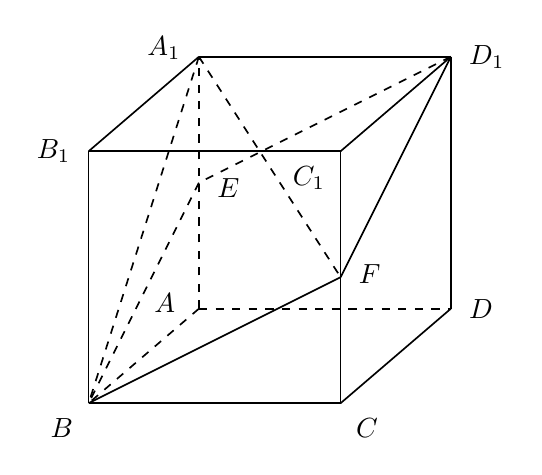
\begin{tikzpicture}[x=1cm,y=1cm,line width=.6pt]
% Cube ABCD-A1B1C1D1; E midpoint of AA1, F midpoint of CC1.
% Base quadrilateral E-B-F-D1 of pyramid A1-EBFD1.
\coordinate (B) at (0,0);
\coordinate (C) at (3.2,0);
\coordinate (D) at (4.6,1.2);
\coordinate (A) at (1.4,1.2);
\coordinate (Bone) at (0,3.2);
\coordinate (Cone) at (3.2,3.2);
\coordinate (Done) at (4.6,4.4);
\coordinate (Aone) at (1.4,4.4);
\coordinate (E) at (1.4,2.8);
\coordinate (F) at (3.2,1.6);
% front face
\draw (B) -- (C);
\draw (C) -- (Cone);
\draw (Cone) -- (Bone);
\draw (Bone) -- (B);
% top face
\draw (Bone) -- (Aone);
\draw (Aone) -- (Done);
% right face
\draw (C) -- (D);
\draw (D) -- (Done);
\draw (Cone) -- (Done);
% hidden bottom/back
\draw[dashed] (A) -- (D);
\draw[dashed] (A) -- (B);
\draw[dashed] (A) -- (Aone);
% hidden depth

% pyramid edges
\draw[dashed] (Aone) -- (B);
\draw[dashed] (Aone) -- (F);
\draw (B) -- (F);
\draw (F) -- (Done);
\draw[dashed] (Done) -- (E);
\draw[dashed] (E) -- (B);


% labels offset clear of strokes
\node[below left,xshift=-2pt,yshift=-2pt] at (B) {$B$};
\node[below right,xshift=2pt,yshift=-2pt] at (C) {$C$};
\node[right,xshift=3pt] at (D) {$D$};
\node[left,xshift=-5pt,yshift=2pt] at (A) {$A$};
\node[left,xshift=-3pt] at (Bone) {$B_{1}$};
\node[below left=2pt] at (Cone) {$C_{1}$};
\node[right,xshift=3pt] at (Done) {$D_{1}$};
\node[left,xshift=-3pt,yshift=3pt] at (Aone) {$A_{1}$};
\node[right,xshift=3pt,yshift=-2pt] at (E) {$E$};
\node[right,xshift=3pt,yshift=1pt] at (F) {$F$};
\end{tikzpicture}
